%%%%%%%%%%%%%%%%%%%%%%%%%%%%%%%%%%%%%%%%%%%%%%%%%%%%%%%%%%%%%%%
% JOURNAL INSTRUCTIONS
% This section may be divided by subheadings and should contain sufficient detail so that when read in conjunction with cited references, all procedures can be repeated. For experiments reporting results on animal or human subject research, an ethics approval statement should be included in this section (for further information, see the Bioethics section.)
%%%%%%%%%%%%%%%%%%%%%%%%%%%%%%%%%%%%%%%%%%%%%%%%%%%%%%%%%%%%%%%

%%%%%%%%%%%%%%%%%%%%%%%%%%%%%%%%%
% Questions for 2021-03-09
% - How should we structure: Experimental Design => Results => Discussion
%   - We conducted 3 separate experiments. Currently, we discuss each experiment separately across sections. (1) do we want to stick to this structure? (2) if so, what should the headings be?
% - What parts of what is currently experimental design belong in methods vs. results. vs discussion?
%   - I 100% want to provide some intuition about measurements (in the paper), but where? I'd like trainees to be able to read this as easily as possible. 
% - I do actually think the details for the metrics/measurements are important. 
% - Discuss the overall flow of the methods section. Should the 'quantifying tape of life' metrics actually be under experiment 1 since that's what they are relevant to?
% - I think we could combine results and discussion? Other major re-organizations?
% - 'mutation accumulation'
%%%%%%%%%%%%%%%%%%%%%%%%%%%%%%%%%

\section{Materials and Methods}

\subsection{The Avida Digital Evolution Platform}

% -- Define digital organisms --
Avida is a study system wherein self-replicating computer programs (digital organisms) compete for space on a finite toroidal grid \citep{ofria_avida:_2009}.
Each digital organism is defined by a linear sequence of program instructions (its genome) and a set of virtual hardware components used to interpret and express those instructions. 
% Avida tracks each organism as it expresses its genome in a given environment in order to measure that organism's phenotype.
Genomes are expressed sequentially except when the execution of one instruction deterministically changes which instruction should be executed next (\textit{e.g.}, a ``jump'' instruction). 
Genomes are built using an instruction set that is both robust (\textit{i.e.}, any ordering of instructions is syntactically valid, though not necessarily meaningful) and Turing Complete (\textit{i.e.}, able to represent any computable function, though not necessarily in an efficient manner).
The instruction set includes operations for basic computations, flow control (\textit{e.g.}, conditional logic and looping), input, output, and self-replication.
% @AML: Outsource the next sentence to a figure!
% The virtual hardware set includes components such as a central processing unit (CPU) for executing instructions, registers to store values, buffers for inputs and outputs, and memory stacks \citep{ofria_avida:_2009}.

% -- Define reproduction & mutation --
Organisms in Avida reproduce asexually by copying their genome instruction-by-instruction and then dividing. 
However, copy operations are imperfect and can result in single-instruction substitution mutations in an offspring's genome. 
For this work, we configured copy operations to err at a rate of one expected mutation for every 400 instructions copied (\textit{i.e.}, a per-instruction error rate of 0.0025).
We held individual genomes at a fixed length of 100 instructions; that is, we did not include insertion and deletion mutations. 
We used fixed-length genomes to control for treatment-specific conditions resulting in the evolution of substantially different genome sizes \citep{supplemental_material}\footnote{
We repeated our experiments without genome size restrictions and observed qualitatively similar results (see supplemental material, \citealt{supplemental_material}).
}, which could, on its own, drive differences in evolutionary outcomes among experimental treatments.
When an organism divides in Avida, its offspring is placed in a random location on the toroidal grid, replacing any previous occupant.
For this work, we used the default 60 by 60 grid size, which limits the maximum population size to 3600 organisms.
As such, improvements to the speed of self-replication are advantageous in the competition for space.

% Avida tracks each organism as it expresses its genome in a given environment in order to measure that organism's phenotype.

% -- Define fitness/metabolic rate/improving replication speed --
During evolution, organism replication rates improve in two ways: by improving genome efficiency (\textit{e.g.}, using a more compact encoding) or by accelerating the rate at which the genome is expressed (their ``metabolic rate'').
An organism's metabolic rate determines the speed at which it executes instructions in its genome.
Initially, an organism's metabolic rate is proportional to the length of its genome, but that rate is adjusted as it completes designated tasks, such as performing Boolean logic computations \citep{ofria_avida:_2009}.
In this way, we can reward or punish particular phenotypic traits. 

% \vspace{0.25cm}
\subsubsection{Phenotypic plasticity in Avida}

% -- Phenotypes & Phenotypic plasticity --
%   - What is a phenotype in Avida?
In this work, we measure a digital organism's phenotype as the set of Boolean logic functions that it performs in a given environment.
Sensory instructions in the Avida instruction set allow organisms to detect how performing a particular logic function would affect their metabolic rate (see supplemental material for more details, \citealt{supplemental_material}). 
We define a phenotypically plastic organism as one that uses sensory information to alter which logic functions it performs based on the environment.

% -- Adaptive plasticity & non-adaptive plasticity --
Phenotypic plasticity in Avida can be adaptive or non-adaptive for a given set of environments.
Adaptive plasticity shifts net task expression closer to the optimum for the given environments.
Non-adaptive plasticity changes task expression in either a neutral or deleterious way. 
Optimal plasticity toggles tasks to always perfectly match the set of rewarded tasks for the given set of environments.

% For the majority of our experiments, we focus on the following 6 one- and two-input logic functions: NOT, NAND, AND, OR-NOT, OR, and AND-NOT. 
% An organism's \textit{comprehensive} or \textit{aggregate} phenotype is characterized by the set of logic functions performed in each of a set of given environments. 

% \vspace{0.7cm}
\subsection{Experimental design}
\label{sec:methods:experiment}

\begin{figure}[h!]
    \centering
    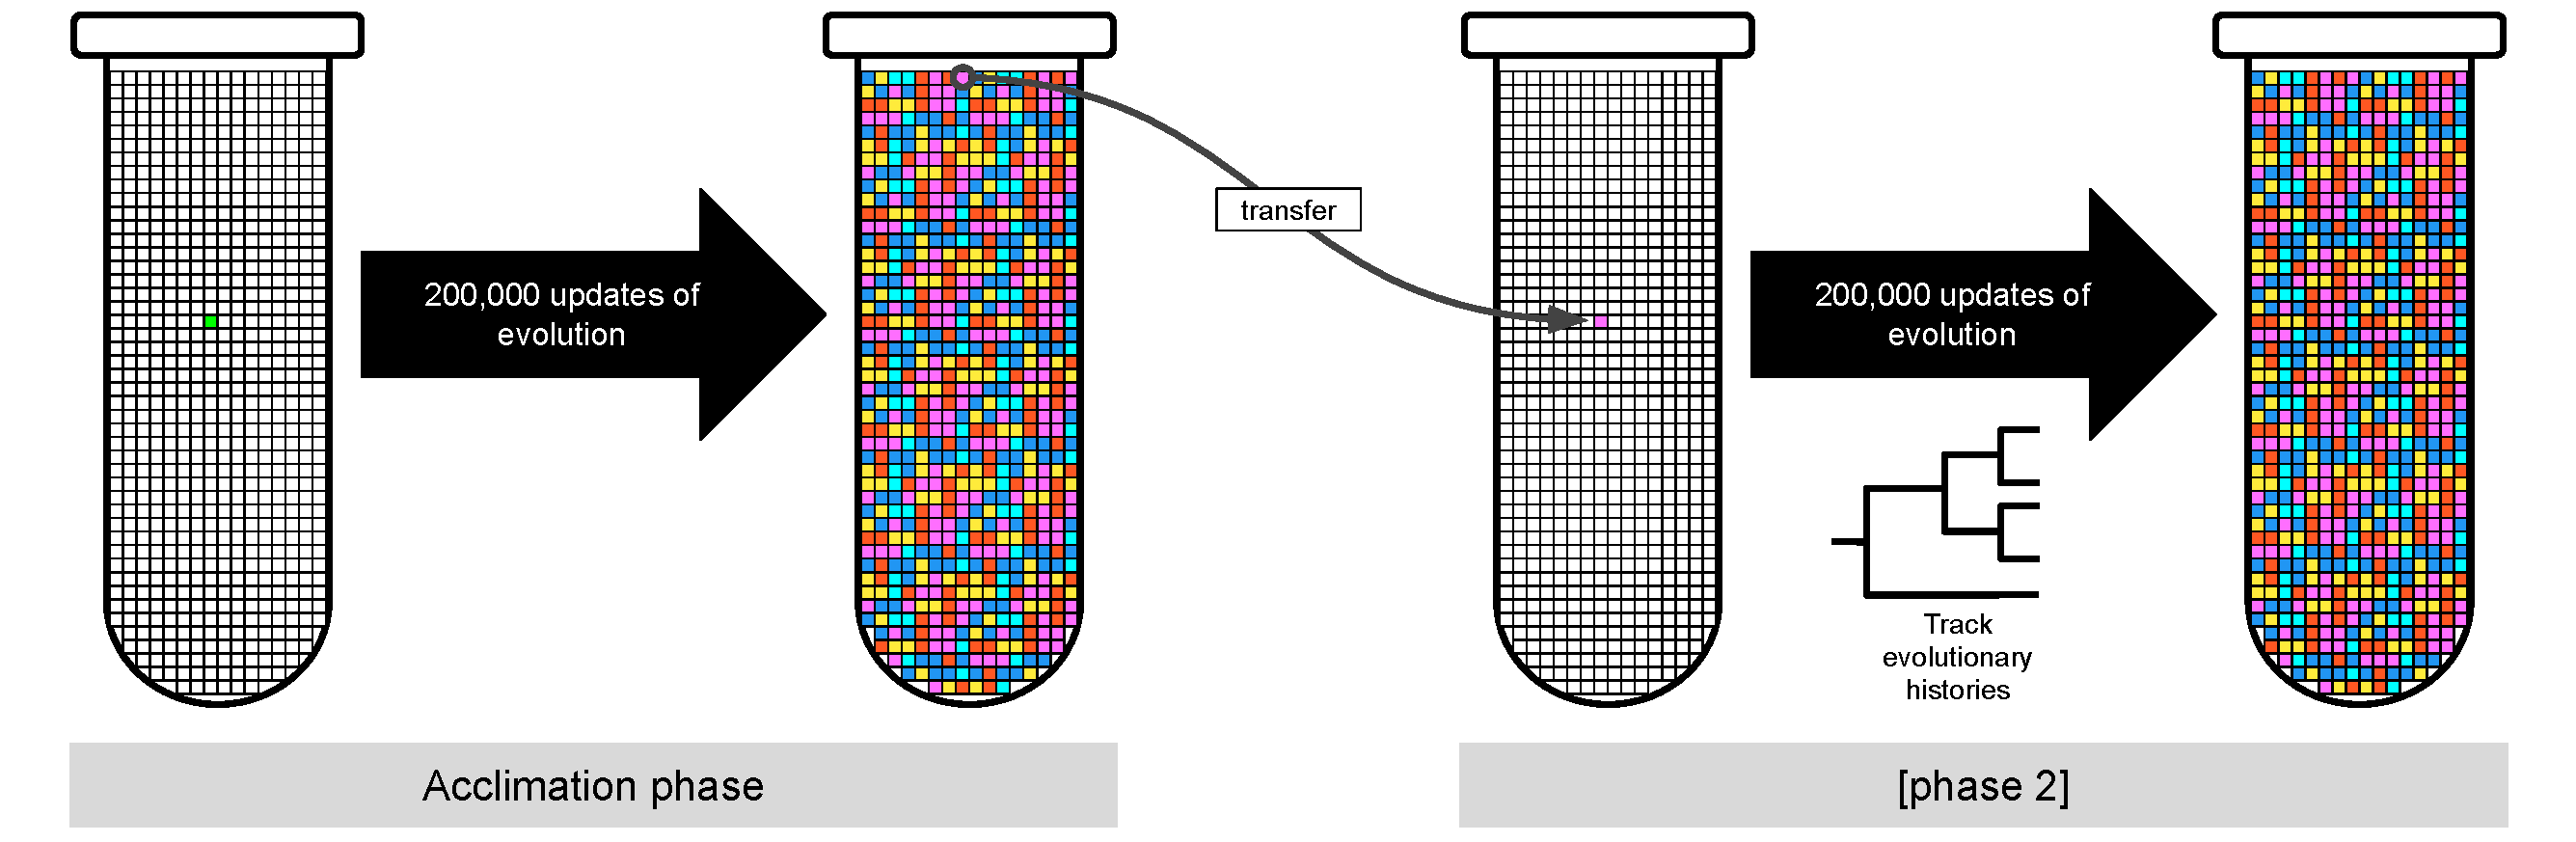
\includegraphics[width=\textwidth]{media/experiment-overview-draft.pdf}
    \caption{\small
    \textbf{todo.}
    todo.
    }
    \label{fig:experimental-design-overview}
\end{figure}

%%%%%%%%%%%%%%%%%%%%%%%%%%%%%%%%%%%%%%%%%%%%%%%%%
% OUTLINE
%%%%%%%%%%%%%%%%%%%%%%%%%%%%%%%%%%%%%%%%%%%%%%%%%
% Overview of experimental design - with diagram (not a subsubsection?)
% - Focused around diagram
% Environment implementations
% Specifications for Phase 1
% specifications for Phase 2A
% specifications for Phase 2B
% specifications for Phase 2C
%%%%%%%%%%%%%%%%%%%%%%%%%%%%%%%%%%%%%%%%%%%%%%%%%

% -- Treatments --
We conducted three independent experiments using Avida to investigate how the evolution of adaptive plasticity influences evolutionary outcomes in fluctuating environments.
For each experiment, we compared the evolutionary outcomes of populations evolved under three treatments (Figure \ref{fig:experimental-design}): 
(1) a \textbf{PLASTIC} treatment where the environment fluctuates, and digital organisms can use sensory instructions to differentiate between environmental states;
(2) a \textbf{NON-PLASTIC} treatment with identical environment fluctuations, but where sensory instructions are disabled;
and (3) a \textbf{STATIC} control where organisms evolve in a constant environment.

% -- Experiment phases --
Each experiment was divided into two phases that each lasted for 200,000 updates\footnote{
    One update in Avida is the amount of time required for the average organism to execute 30 instructions. 
    See \citep{ofria_avida:_2009} for more details.
} of evolution (Figure \ref{fig:experimental-design}), which is approximately 30,000 to 40,000 generations.
In phase one of each experiment, we preconditioned populations to their treatment-specific conditions.
In phase two, we founded new populations with the evolved organisms from phase one and examined their subsequent evolution under given combinations of treatment and experimental conditions.
During phase two, we tracked each population's evolutionary history as well as saving the full final population.
Phase one was for pre-conditioning only; all comparisons between treatments were performed on phase two data.

% \vspace{0.25cm}
\vspace{5mm}
\subsubsection{Environments}
\label{sec:methods:experiment:environments}

% ----- ENVIRONMENTS -----
% traits_set_a <- c("not", "and", "or")
% traits_set_b <- c("nand", "ornot", "andnot")

% -- Environment definitions --
We constructed three experimental environments, abbreviated hereafter as ``ENV-A'', ``ENV-B'', and ``ENV-ALL''.
Figure [YY] describes these environments based on whether each of six Boolean logic tasks (NOT, NAND, AND, OR-NOT, OR, and AND-NOT) is rewarded or punished.
A rewarded task performed by an organism doubles their metabolic rate, allowing them to execute twice as many instructions in the same amount of time.
A punished task halves an organism's metabolic rate. 


% --- TODO - Move these descriptions to the figure caption ---
% In ENV-A, organisms are rewarded for performing NOT, AND, and OR, but are punished for performing the NAND, OR-NOT, and AND-NOT logic tasks.
% Conversely in ENV-B, organisms are rewarded for performing NAND, OR-NOT, and AND-NOT, but are punished for performing NOT, AND, and OR. 
% Finally, in ENV-ALL, all six tasks are rewarded and none are punished.

% @AML: Add deleted text to figure caption.
% Organisms with phenotypes that align with their current environment will quickly outcompete those with mismatched phenotypes.  
% A perfect match in ENV-A or ENV-B will have a metabolic bonus of $\times{8}$, a perfect mismatch will have a penalty of $\times{0.125}$, and an organism that does no tasks or all tasks will not have a modifier at all. 
% ------------------------------------------------

% -- Treatment-specific environment details --
In both the PLASTIC and NON-PLASTIC conditions, the environment cycles between equal-length periods of ENV-A and ENV-B.
Each of these periods persist for 100 updates (approximately 15 to 20 generations).
Thus, populations experience a total of 1,000 full periods of ENV-A interlaced with 1,000 full periods of ENV-B during each experimental phase.

% -- Sensory instructions + control flow and controlling the capacity for plasticity --
Organisms in the PLASTIC treatments differentiate between ENV-A and ENV-B by executing one of six sensory instructions, each associated with a particular logical task; these sensory instructions detect whether their associated task is currently rewarded or punished.
By using sensory information in combination with execution flow-control instructions, organisms can conditionally perform different logic tasks depending on the current environmental conditions.

\vspace{5mm}
\subsubsection{Experiment Phase 1 -- Environment preconditioning}
\label{sec:methods:experiment:phase-one}
% @AML: if we use 'phase 1' and 'phase 2X' in headings, should we switch all 'phase one' text to 'phase 1' etc?

For each treatment, we founded 100 independent populations from a common ancestral strain capable only of self-replication.
At the end of phase one, we identified the most abundant (\textit{i.e.}, dominant) genotype and extracted an organism with that genotype from each replicate population to found a new population for phase two.

%The evolution of adaptive phenotypic plasticity is not a guaranteed outcome in phase one of the PLASTIC treatment.
For the PLASTIC treatment, we measure plasticity by independently testing a given genotype in each of ENV-A and ENV-B.
We discard phase one populations if the dominant genotype does not exhibit optimal plasticity.
This approach ensures that measurements taken on PLASTIC-treatment populations during the second phase of each experiment reflect the evolutionary consequences of adaptive plasticity.

\vspace{5mm}
\subsubsection{Experiment Phase 2A -- Evolutionary change rate}
\label{sec:methods:exp:evolutionary-change-rate}

Phase 2A continued exactly as phase one, except we tracked the rates of evolutionary change in each of the PLASTIC-, NON-PLASTIC-, and STATIC-treatment populations. 
Specifically, we quantified evolutionary change rates using four metrics (each described in Table~\ref{tab:metrics-definitions}):
(1) coalescence event count,
(2) mutation count, 
(3) phenotypic volatility,
% (4) genotypic fidelity, 
% (5) phenotypic fidelity,
and (4) mutational stability.
We additionally used knockout experiments to examine how the genetic architectures of organisms and their ancestors changed over time.

\vspace{3mm}
\subsubsection{Experiment Phase 2B -- Novel task evolution}
\label{sec:methods:exp:novel-task-evolution}

Phase 2B extended the conditions of phase one by adding 71 novel Boolean logic tasks, which were always rewarded in all treatments \citep{ofria_avida:_2009}.
The original six phase one tasks (NOT, NAND, AND, OR-NOT, OR, and AND-NOT; hereafter called ``base'' tasks) continued to be rewarded or punished according to the particular treatment conditions.
% @CAO: line below can be restored (and reworded) if readers need help with the intuition.
%As such, in fluctuating environments, the six base tasks continued to fluctuate, but the additional 71 tasks were always rewarded; in static environments, performing any of the 77 logic tasks was always beneficial.
An organism's metabolic rate was increased by \novelTraitsReward\ for each novel task that it performed (limited to one reward per task).
This reward provided a selective pressure to evolve these tasks, but their benefits did not overwhelm the 100\% increase conferred by rewarded base tasks. 
As such, populations in the PLASTIC and NON-PLASTIC treatments could not easily escape environmental fluctuations by abandoning the fluctuating base tasks.

During this experiment, we tracked the extent to which populations evolving under each treatment were capable of acquiring and retaining novel tasks.  
Specifically, we used three metrics (each described in Table~\ref{tab:metrics-definitions}):
(1) final novel task count,      % WAS: task performance
(2) novel task discovery,    % WAS: task discovery
and (3) novel task loss. % WAS: task loss

\vspace{5mm}
\subsubsection{Experiment Phase 2C -- Deleterious instruction accumulation}
\label{sec:methods:exp:deleterious-instruction-accumulation}

% Phase 2C extended the conditions of phase 1 by adding a single ``poisonous'' task, which is always harmful in all treatments.
Phase 2C extended the instruction set of phase one with a \code{poison} instruction.
When an organism executes a \code{poison} instruction, it performs a ``poisonous'' task, which reduces the organism's metabolic rate (and thus reproductive success) but does not otherwise alter the organism's function.
We imposed a 10\% penalty each time an organism performed the poisonous task, making the \code{poison} instruction explicitly deleterious to execute.
We did not limit the number of times that an organism could perform the poisonous task, and as such, organisms could perform the poisonous task as many times as they executed the \code{poison} instruction. 

We tracked the number of times each organism along the dominant lineage performed the poisonous task.
Specifically, we used two metrics (each described in Table~\ref{tab:metrics-definitions}):
(1) final poisonous task count,
and (2) poisonous task acquisition.


% --- POISON INSTRUCTION LANGUAGE --- 
% Phase 2C extended the instruction set of phase one with a \code{poison} instruction.
% When executed by an organism, the \code{poison} instruction reduces the organism's metabolic rate (and thus reproductive success), but does not otherwise alter the organism's function.
% We imposed a 10\% penalty each time an organism executed the \code{poison} instruction, making the instruction explicitly deleterious.
% We tracked the number of times a \code{poison} instruction was executed by each genotype along the dominant lineage (including the final dominant genotype).
% Specifically, we used two metrics (each described in Table~\ref{tab:metrics-definitions}):
% (1) final \code{poison} count,
% and (2) lineage \code{poison} count.

% - measurements -
% @AML: This could get moved to the results?
% At the beginning of phase two, the \code{poison} instruction is not present in the population as it was not part of the instruction set during the first phase of evolution.
% However, by adding \code{poison} to the instruction set during phase two, it can be introduced via a mutation.
% We measured deleterious mutation accumulation by examining the number of times a \code{poison} instruction is executed by each genotype along the dominant lineage (including the final dominant genotype).
% Because the \code{poison} instruction is explicitly deleterious, selection should purge mutations that increase \code{poison} execution in the offspring phenotype.
% As such, we expected such mutations to show up in successful lineages either as accumulated cryptic variation in plastic genomes or via hitchhiking with linked beneficial mutations [cite].

\vspace{5mm}
\subsection{Experimental analyses}

% Evolutionary history

% Lineages and phylogenies
% - number of coalescence
% - mutation accumulation
% - phenotypic volatility
% - mutational stability
% - novel task performance
% - novel task discovery
% - genetic architectures


% TODO - edit descriptions in figure. 
% TODO - coalescence rate as a metric?
% TODO - lineage novel task count => lineage novel task discovery? We take a rate for this eventually, and it's awkward to say 'per-generation lineage novel task count'.
% TODO - lineage poison count => lineage poison increases?
%%%%%%%%% BOX %%%%%%%%%%%%
% this is my current "definition" environment
% \newtcolorbox[auto counter]{definitions}[1][] {
%   enhanced,
%   breakable,
%   arc=0mm,
%   title={\textbf{Box \thetcbcounter. Metrics}},
%   #1
% }

% \begin{definitions}[colback=blue!5!white,colframe=blue!75!black,label=box:metrics]

% Hello world.

% \end{definitions}
%%%%%%%%%%%%%%%%%%%%%%%%%%

% @AML: Not sure the best way to start the description of each metric. 

\newcommand{\SweepsMetricName}{
Coalescence event count
}
\newcommand{\SweepsMetricDesc}{
Number of coalescence events that have occurred, which indicates the frequency of selective sweeps in the population.
}

\newcommand{\MutationCountMetricName}{
Mutation count
}
\newcommand{\MutationCountMetricDesc}{
Sum of all mutations that have occurred along a lineage.
}

% Phenotypic volatility => 
% - 
\newcommand{\PhenotypicVolatilityMetricName}{
Phenotypic volatility
}
\newcommand{\PhenotypicVolatilityMetricDesc}{
Number of instances where parent and offspring phenotypic profiles do not match along a lineage.
% Phenotypic volatility as defined here indicates the rate at which accumulated genetic changes actually change the phenotype along a lineage.
}

\newcommand{\MutationalStabilityMetricName}{
Mutational robustness
% OLD: Mutational stability
}
\newcommand{\MutationalStabilityMetricDesc}{
Proportion of mutations (from the set of all possible one-step mutations) that do not change the phenotypic profile of a focal genotype. We also measured \textit{realized mutational robustness}, which is the proportion of mutated offspring along a lineage whose phenotypic profile matches that of their parent. 
% OLD DEFS:
% - Proportion of mutated offspring along a lineage whose phenotypic profile matches that of their parent. 
% - Proportion of mutants whose phenotypic profile matches that of their parent. Two variations were recorded: lineage mutational stability which examines the mutated offspring along a lineage, and neighborhood mutational stability which examines a set of possible mutations on a given genotype.
}


% Mutational stability => phenotypic stability / mutational robustness
% - Lineage => realized phenotypic stability / realized stability / realized mutational robustness
% - Neighborhood => potential phenotypic stability / potential stability / potential mutational robustness

% - Mutational robustness
% - Realized mutational robustness

\newcommand{\TaskPerformanceMetricName}{
Final novel task count
}
\newcommand{\TaskPerformanceMetricDesc}{
Count of unique novel tasks performed by the representative organism in a final population from experiment \hyperref[sec:methods:exp:novel-task-evolution]{phase 2B}. 
This metric can range from 0 to 71 and measures how well the fitness landscape was exploited  at a given point in time.
% (\textit{i.e.}, the mapping between genetic space and phenotype space)
% We focused on an organism from the dominant genotype at the end of the experiment as the most representative phenotype in the evolved population.
% Final task count is equivalent to the ``task performance'' metric in \citep{canino-koning_fluctuating_2019}.
}

\newcommand{\TaskDiscoveryMetricName}{
Novel task discovery
}
\newcommand{\TaskDiscoveryMetricDesc}{
Number of unique novel tasks ever performed along a given lineage in experimental \hyperref[sec:methods:exp:novel-task-evolution]{phase 2B}, even if a task is later lost.
This metric can range from 0 to 71 and measures a given lineage's level of exploration of the fitness landscape.
}

\newcommand{\TaskLossMetricName}{
Novel task loss
}
\newcommand{\TaskLossMetricDesc}{
Number of instances along a given lineage from experimental \hyperref[sec:methods:exp:novel-task-evolution]{phase 2B} where a novel task is performed by a parent but not its offspring. 
This metric measures how often a given lineage fails to retain evolved traits over time.
}

\newcommand{\FinalPoisonMetricName}{
Final poisonous task count
}
\newcommand{\FinalPoisonMetricDesc}{
Number of times the poisonous task is performed by the representative organism from a final population from experiment \hyperref[sec:methods:exp:deleterious-instruction-accumulation]{phase 2C}.
}

\newcommand{\LineagePoisonMetricName}{
Poisonous task acquisition count
}
\newcommand{\LineagePoisonMetricDesc}{
Number of instances along a given lineage where a mutation causes an offspring to perform the poisonous task more times than its parent. 
}

\newcommand{\ArchitectureVolatilityMetricName}{
Architectural volatility
}
\newcommand{\ArchitectureVolatilityMetricDesc}{
The average number of loci in the genome that change function per mutation along a lineage. 
% @AML: The average number of mutations that cause a change in function along a lineage. 
%Loci function is denoted as the combination of task machinery, plasticity machinery, vestigial machinery for both ENV-A and ENV-B tasks, as well as replication and required machinery. 
}

\newcommand*{\thead}[1]{\multicolumn{1}{c}{\bfseries #1}}

\setlength{\tabcolsep}{16pt}
\renewcommand{\arraystretch}{1.5}
\begin{table}[ht]
    \centering
    
    \rowcolors{2}{gray!25}{white}
    \begin{tabularx}{\linewidth}{lX} % p{10cm}
        \rowcolor{gray!50}
        \hline 
        \thead{Metric} & \thead{Description}   \\
        \hline
        \SweepsMetricName & \SweepsMetricDesc \\
        \MutationCountMetricName & \MutationCountMetricDesc \\
        \PhenotypicVolatilityMetricName & \PhenotypicVolatilityMetricDesc \\
        % \GenotypicFidelityMetricName &         \GenotypicFidelityMetricDesc \\
        % \PhenotypicFidelityMetricName &         \PhenotypicFidelityMetricDesc \\
        \MutationalStabilityMetricName & \MutationalStabilityMetricDesc \\
        % (architecture metric(s)) & \\
        %\ArchitectureVolatilityMetricName & \ArchitectureVolatilityMetricDesc \\
        \TaskPerformanceMetricName & \TaskPerformanceMetricDesc \\
        \TaskDiscoveryMetricName & \TaskDiscoveryMetricDesc \\
        \TaskLossMetricName & \TaskLossMetricDesc \\
        \FinalPoisonMetricName & \FinalPoisonMetricDesc \\
        \LineagePoisonMetricName & \LineagePoisonMetricDesc \\
        \hline
    \end{tabularx}
    
    \caption{\textbf{Metric descriptions.}}
    \label{tab:metrics-definitions}
\end{table}




% naive environment = what organism experiencing
% alternative environment = what organism is not currently experiencing

% - How we extracted representative lineages -
For each of our experiments, we tracked and analyzed the phylogenetic histories of evolving populations during phase two. 
For each replicate, we identified an organism with the most abundant genotype in the final evolved population that we used as a representative organism for further analysis.
We then isolated the lineage from the founding organism to the representative organism, which we used as the representative lineage for further analysis.
We manually inspected evolved phylogenies and found no evidence that any of our experimental treatments supported long-term coexistence. 
As such, each of the representative lineages reflect the majority of evolutionary history from a given population at the end of our experiment.
%Because our experimental treatments do not support long-term coexistence, each of these lineages represented the majority of evolutionary history from a given population at the end of our experiment.

% -- PHENOTYPIC PROFILE --
% DEFINE PHENOTYPIC PROFILE - metric definitions will use this.
Some of our metrics required us to measure genotype-by-environment interactions.
Importantly, in the fluctuating environments, we needed to differentiate phenotypic changes that were caused by mutations from those that were caused by environmental changes.
To accomplish this task, we produced organisms with the focal genotype, measured their phenotype in each environment, and aggregated the resulting phenotypes to create a \textit{phenotypic profile}. 
Although organisms with different genotypes may express the same set of tasks across environments, their phenotypic profiles may not necessarily be the same.
For example, an organism that expresses NOT in ENV-A and NAND in ENV-B has a distinct profile from one that expresses NAND in ENV-A and NOT in ENV-B.

% ---- group editing - BOOKMARK ----

% -- KNOCKOUT EXPERIMENTS --
% While Avida clearly defines the mechanics of each instruction, the emergent function of an instruction depends on its context within a genome. 
For an individual organism, we can perform knockout experiments to identify which instructions are responsible for producing a given phenotypic outcome.
To perform a knockout, we duplicate the organism, replacing a single instruction with an inert ``no-operation'' instruction.
We then identify any phenotypic changes by contrasting the execution results of the ``knockout'' organism and the original.
Such changes provide evidence of the role that the original instruction must have played in the genome.
For example, when an organism performs the NAND task but loses it when an instruction is knocked out, we categorize that instruction as part of the NAND task machinery.
% @AML: maybe move next sentence to results?
We use knockout experiments to characterize the role of each instruction in the genomes of every organism along all study lineages, revealing how genetic architectures change over time.


%%%%%%%%%%%%%%%%%%%%%%%%%%%%%%%%%%%%%%%%%%%%%%%%%%%%%%%%%%%%%%%%%%%%%%%%%%%%%%%%%%%%%%%%%%%%%%%%%%%%%%%%%%%%%%%%

% - Measuring evolutionary change -
% We quantified rates of evolutionary change using the following four metrics (Box \ref{box:metrics}):
% (1) number of \textbf{coalescence events} that have occurred, which indicates the frequency of selective sweeps in the population;
% (2) \textbf{mutation accumulation}, which is the sum of all mutations that have occurred along a lineage;
% (3) \textbf{phenotypic volatility}, which is the number of instances where parent and offspring phenotypes do not match along a lineage, as measured under a given condition;
% and (4) \textbf{mutational stability}, which is the proportion of \textit{mutated} offspring along a lineage whose phenotypes do not match that of their parent, as measured under a given condition.

% - Methods for computing volatility -
% To calculate phenotypic volatility for a given lineage, we expressed (i.e., evaluated) each genotype along that lineage in a treatment-specific condition, and we summed the number of changes in task profiles between consecutive genotypes.
% For lineages evolved in environments fluctuating between ENV-A and ENV-B, we evaluate genotypes in both environmental conditions and count only changes in its \textit{aggregate} phenotype; this technique ensures that environmentally-induced changes are excluded from our measurement.
% Phenotypic volatility as defined here illuminates the rate at which accumulated genetic changes actually change the phenotype along a lineage.

% - Methods for computing mutational stability
% We measured mutational stability as the fraction of mutated offspring along a given lineage with a different phenotype than their parent.
% For lineages evolved in fluctuating environments, we evaluated mutants under both ENV-A and ENV-B and counted all changes in the \textit{aggregate} task profile; like our measure of phenotypic volatility, this technique ensures that environmentally-induced changes are excluded from our measurement.
% Mutational stability examines the frequency at which mutations effect changes in an offspring's phenotype.
 
% In experiments that introduce novel tasks during phase two, we measured task discovery, task performance, and task loss along representative lineages.
% \textbf{Task discovery} measures a given lineage's level of \textit{exploration} of the fitness landscape (i.e., the mapping between genetic space and phenotype space) \citep{canino-koning_fluctuating_2019}. 
% We calculated task discovery as the total number of unique tasks ever performed along the lineage, even if a task is later lost; as such, a lineage's task discovery measurement ranged from 0 to 71.

% \textbf{Task performance} measures the level of \textit{exploitation} of the fitness landscape at a given point in time.
% In this work, we summarized task performance using a count of unique tasks completed by a representative organism from each population.
% We focused on an organism from the dominant genotype at the end of the experiment as the most representative phenotype in the evolved population.

% \textbf{Task loss} measures how often a lineage fails to retain evolved traits over time and thus indicates the ability for traits to be maintained over time.
% We calculated task loss as the number of times along a lineage that a task is performed by a parent but not its offspring. 

% \textbf{Final poison count}...

% \textbf{Lineage poison count}...

%%%%%%%%%%%%%%%%%%%%%%%%%%%%%%%%%%%%%%%%%%%%%%%%%%%%%%%%%%%%%%%%%%%%%%%%%%%%%%%%%%%%%%%%%%%%%%%%%%%%%%%%%%%%%%%%


% \vspace{0.5cm}
\vspace{5mm}
\subsection{Statistical analyses}

Across all of our experiments, we differentiated between sample distributions using non-parametric statistical tests.
For each major analysis, we first performed a Kruskal-Wallis test \citep{kruskal_use_1952} to 
determine if there were significant differences in results from the PLASTIC, NON-PLASTIC, and STATIC treatments (significance level $\alpha=0.05$).
If so, we applied a Wilcoxon rank-sum test \citep{kotz_individual_1992} to distinguish between pairs of treatments.
We applied Bonferroni corrections for multiple comparisons \citep{rice_analyzing_1989} where appropriate.

\vspace{5mm}
\subsection{Software availability}

We conducted our experiments using a modified version of the Avida software, which is open source and freely available on \href{https://github.com/amlalejini/evolutionary-consequences-of-plasticity}{GitHub} \citep{supplemental_material}.
We used Python for data processing, and we conducted all statistical analyses using R version 4 \citep{r_core_team_r_v4}.
We used the tidyverse collection of R packages \citep{r_tidyverse_2019} to wrangle data, and we used the following R packages for analysis, graphing, and visualization: 
ggplot2 \citep{R-ggplot2}, 
cowplot \citep{R-cowplot}, 
Color Brewer \citep{harrower_colorbrewerorg_2003,R-Brewer_2014}, 
rstatix \citep{R-rstatix},
ggsignif \citep{R-ggsignif},
scales \citep{R-scales},
Hmisc \citep{R-Hmisc}, 
fmsb \citep{R-fmsb}, 
and boot \citep{R-boot}.
We used R markdown \citep{rmarkdown} and bookdown \citep{R-bookdown} to generate web-enabled supplemental material.
All of the source code for our experiments and analyses, including guides for replication and configuration files, can be found in our supplemental material, which is hosted on \href{https://github.com/amlalejini/evolutionary-consequences-of-plasticity}{GitHub} \citep{supplemental_material}.
Additionally, our experimental data is available on the Open Science Framework at \url{https://osf.io/sav2c/} \citep{osf_data}.